Theorems used in the set (for reference):
\begin{numberedthm}{3.10}\label{thm:3.10}
There exists a function $f(n)$ with the following property: if $f(n)$ points of the plane are in general position (no three on a line) then there exists $n$ of these points forming the vertices of a convex $n$-\textup{gon}.
\end{numberedthm}

\subsection*{Problem 11}
Show that the $n$-element sets of a $(2n+k)$-element ground set can be partitioned into $k+2$ classes so that each class contains pairwise intersecting sets.

\begin{proof}
Suppose the ground set is $[2n+k]=\{1,2,\dots,2n+k\}$. Consider all $n$-element subsets of $[2n+k]$. To do so, we will define a proper coloring of the Kneser graph $\text{KG}(2n+k,n)$ with $k+2$ colors. Then, the color classes pairwise intersecting sets. To perform such a coloring, give color $i$ to every $n$-subset who's smallest element is $i$ for every $i \in [k+1]$. Note that this uses at most $k+1$ colors. Then, give color $k+2$ for all other $n$-subsets. Through this coloring, we have used $k+2$ colors in total. This coloring is a proper coloring since if two $n$-element sets have the same color $i \leq k+1$, then they must have the same minimum element $i$, and so they are not disjoint and thus, cannot be adjacent in the Kneser graph. This means that any set with a color $i \in [k+1]$ is independent in the Kneser graph. Now, note that every $n$-set colored $k+2$ is in the set $\{k+2,k+3\dots,2n+k\}$, which has $2n-1$ elements. Note that any $n$-subset of a $2n-1$-set is intersecting due to the Pigeonhole Principle, and thus, sets colored $k+2$ are also independent in the Kneser graph. We have then colored this Kneser graph with $k+2$ colors, and thus, the $n$-element sets of a $(2n+k)$-element ground set can be partitioned into $k+2$ classes so that each class contains pairwise intersecting sets.
\end{proof}

\subsection*{Problem 12}
Let $t$ be a positive integer. Construct a 2-chromatic (bipartite) graph $G$ such that for some ordering of the vertices of $G$, the greedy algorithm uses $t$ colors for coloring $G$.

\begin{proof}
Suppose $t=2$. Consider a 2 vertex graph with one edge connecting the root to its leaf. For the greedy algorithm, order the leaf before the root. Clearly, we need 2 colors to color $G$ through such a greedy algorithm, which is exactly $t$. For $t=3$, consider two copies of the $t=2$ case, and connect the roots. Order the leafs (vertices with degree 1) before their parents, which are the root in this case. Since one of the roots are are adjacent to both the leafs and the other root, it requires a third unique color, and thus, we need 3 colors to color $G$, which is exactly $t$. Through this process of considering 2 copies of the previous case and connecting the roots, we can construct a tree. Note that for any $t$, if we allow the roots of two trees of the $t-1$ case to be adjacent by adding an edge between them, we construct another tree who has two "parent" vertices, both of which have the same color when such an edge is added, and thus, requires one of them to adopt a unique color, leading to $t$ colors to color the graph. Note that since we construct trees, the graph $G$ is always bipartite.
\end{proof}

\subsection*{Problem 13}
Prove that $R(3,4)=9$

\begin{proof}
% TODO: Show $R(3,4) \leq 9$ and $R(3,4) \geq 9$
First, note that $R(3,4) \geq 9$. Below is a colored $K_8$ with edges either red or blue. Note that there are no blue colored $K_3$ subgraphs nor red colored $K_4$ subgraphs. 
\begin{center}
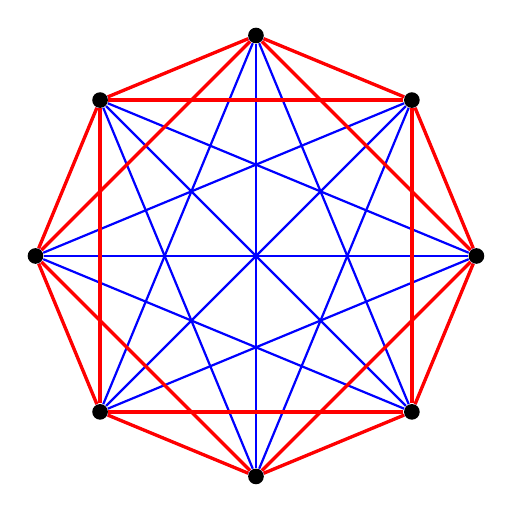
\begin{tikzpicture}[scale=2, every node/.style={circle, fill, inner sep=2pt, draw=none}]
    \foreach \i/\ang in {1/0,2/45,3/90,4/135,5/180,6/225,7/270,8/315}{
        \node (v\i) at (\ang:1.4) {};
    }

    \foreach \i in {1,...,8}{
        \foreach \j in {1,...,8}{
        \ifnum\i<\j
            \draw[blue, thick] (v\i) -- (v\j);
        \fi
        }
    }
    \draw[red, very thick] (v1) -- (v2);
    \draw[red, very thick] (v2) -- (v3);
    \draw[red, very thick] (v3) -- (v4);
    \draw[red, very thick] (v4) -- (v5);
    \draw[red, very thick] (v5) -- (v6);
    \draw[red, very thick] (v6) -- (v7);
    \draw[red, very thick] (v7) -- (v8);
    \draw[red, very thick] (v8) -- (v1);

    \draw[red, very thick] (v1) -- (v3);
    \draw[red, very thick] (v2) -- (v4);
    \draw[red, very thick] (v3) -- (v5);
    \draw[red, very thick] (v4) -- (v6);
    \draw[red, very thick] (v5) -- (v7);
    \draw[red, very thick] (v6) -- (v8);
    \draw[red, very thick] (v7) -- (v1);
    \draw[red, very thick] (v8) -- (v2);

\end{tikzpicture}
\end{center}
Thus, $R(3,4) \geq 9$.
Now we shall show that $R(3,4) \leq 9$.
\end{proof}

\subsection*{Problem 14}
Show that $2^r < R(\underbrace{3,3,\dots,3}_\text{$r$}) \leq 3r!$
\begin{proof}
First, we will show  $2^r < R(3,3,\dots,3)$. Suppose we have a graph with $r$ vertices. Enumerate each vertex with a binary $r$-digit number. An edge is colored corresponding to the first differing digit between two vertices. Now, consider a triangle ($K_3$) inside of this graph. If 2 vertices differ at position, then the third vertex cannot be enumerated in this way. Since this construction is impossible, we cannot have this binary vertex enumeration, and thus, we must have strictly more than $2^r$ vertices. Thus, $2^r < R(3,3,\dots,3)$ Finally, we will show $R(3,3,\dots,3) \leq 3r!$. Consider the graph with $K_{3r!}$ with $3r!$ vertices. For a first vertex, it must be connected to $3r!-1$ other vertices. Since there are $r$ colors, by the Pigeonhole Principle, each edge is connected to at least $3(r-1)!$ other vertices. Now continue this process by considering another color, which then has $3(r-2)!$ it is connected to. Continue this process until we have $3$ vertices left, which cannot be colored monochromatically without there existing a monochromatic $K_3$, and thus, $R(3,3,\dots,3) \leq 3r!$

\end{proof}

\subsection*{Problem 15}
Show that $R_3(n,n)$ is also a good choice for $f(n)$ in \autoref{thm:3.10} (Hint: color a triple of points $\{a,b,c\}$ according to the parity of the number of points inside the triangle $abc$.)

\begin{proof}
We will show that if $R_3(n,n)$ points of the plane are in general position, then there exists $n$ of these points forming the vertices of a convex $n$-gon. Let $N \in \mathbb{Z}_{>0}$, and consider the set $P=p_1, \dots, p_N$ in general position. Now consider all triples $\{a,b,c\}$ in P and color the triple red if the number of points of $P$ are inside the triangle and is even and blue if odd. If $N \geq R_3(n,n)$, then we know that there is a monochromatic $n$-subset in $P$. We can call this subset $A$. If all triples in $A$ are monochromatic, then no point of $A$ lies in the convex hull of the others, and thus, the $n$ points in $A$ form a convex $n$-gon.
\end{proof}